\begin{center}
\begin{tikzpicture}[x=1cm,y=1cm]
%\pgfresetboundingbox
\draw[use as bounding box, anchor = north west,draw,dashed,gray] (-5.5,-3.25) rectangle (5.5,3.25);
\clip (-5.5,-3.25) rectangle (5.5,3.25);
\node[anchor =north west] (text) at (-5.25,3.25){\begin{minipage}{5.0cm}
\visible<1-8>{Let us use \textbf{polynomials} to estimate:}
\begin{align*}
    y(x) &=\sin(2\pi x)
\end{align*}
Note that $f^{*} \notin \mathcal{T}$!\\
\only<2>{Assume $8$ measurements with noise $\mathcal{N}(0,0.2)$}\\
\only<3-4>{Start with degree $2$...\only<4>{What happens when we increase the order?}}
\only<6-8>{\\ What do the risk terms look like?}
\only<8->{\vspace{1.75cm}\\\color{red}{What happens if we add more data?}}
\end{minipage}};
\visible<1>{\node (figure) at (2.75,0){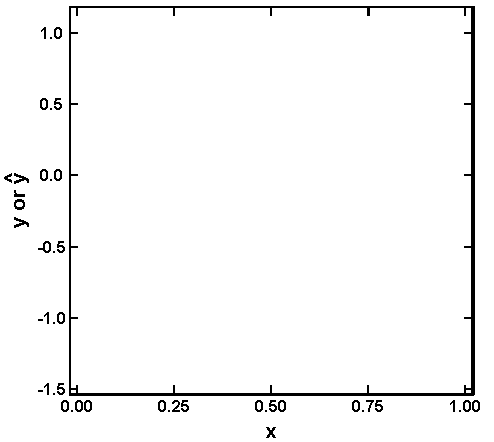
\includegraphics[width=5cm]{satistical_learning/figures/comp_1.pdf}};}
\visible<2>{\node (figure) at (2.75,0){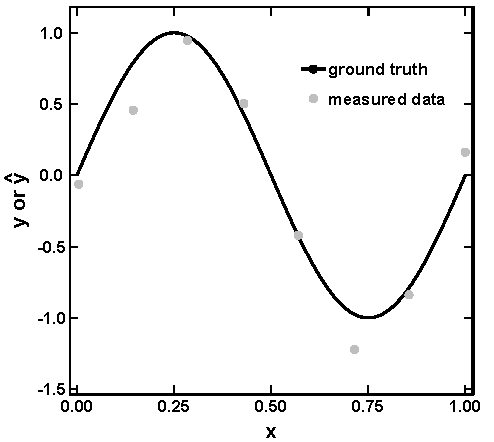
\includegraphics[width=5cm]{satistical_learning/figures/comp_2.pdf}};}
\visible<3>{\node (figure) at (2.75,0){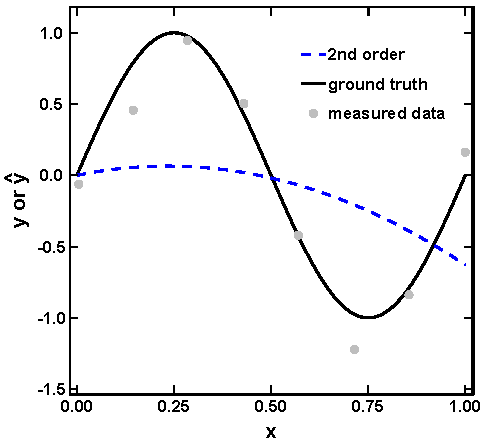
\includegraphics[width=5cm]{satistical_learning/figures/comp_3.pdf}};}
\visible<4>{\node (figure) at (2.75,0){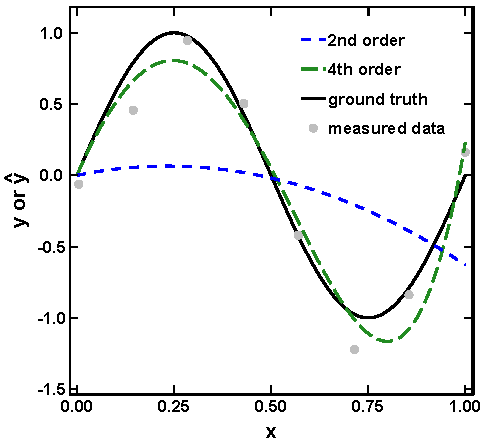
\includegraphics[width=5cm]{satistical_learning/figures/comp_4.pdf}};}
\visible<5-6>{\node (figure) at (2.75,0){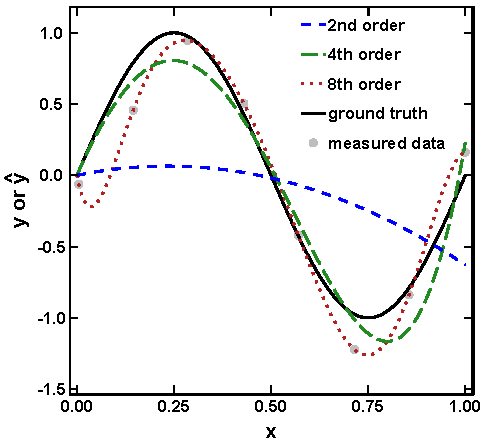
\includegraphics[width=5cm]{satistical_learning/figures/comp_5.pdf}};}
\visible<7->{\node (figure) at (2.75,0){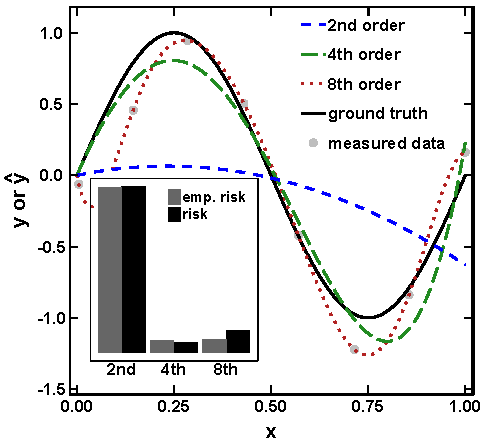
\includegraphics[width=5cm]{satistical_learning/figures/comp_6.pdf}};}
\visible<9->{\node (figure) at (-2.75,0){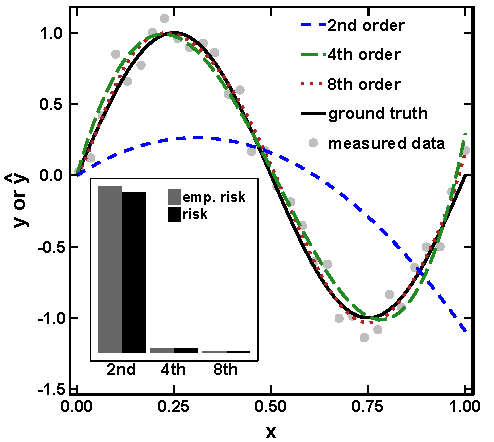
\includegraphics[width=5cm]{satistical_learning/figures/comp_lots_6.pdf}};}
\end{tikzpicture}
\end{center}